\documentclass[a4paper,11pt]{article}
\usepackage[left=3cm,top=3cm,right=2cm,bottom=2cm]{geometry}
\usepackage[brazilian, english]{babel}
\usepackage[utf8]{inputenc}
\usepackage[numbers]{natbib}
\usepackage{epigraph}
\usepackage{indentfirst}
\usepackage{listings}
\usepackage{graphicx}
\usepackage{wrapfig}
\usepackage{setspace}
\usepackage[hidelinks]{hyperref}
\usepackage[bottom]{footmisc}
%\usepackage{xcolor}
\usepackage[dvipsnames]{xcolor}
\usepackage{adjustbox}
\usepackage{verbatim}
\usepackage{float}
\usepackage{lmodern}% http://ctan.org/pkg/lm
\usepackage{svg}
\newcommand{\tabitem}{~~\llap{\textbullet{\ensuremath{\bullet}}}~~}
\newcommand*{\SignatureAndDate}[4]{%
	\parbox{7cm}{
      \centering
      \rule{6cm}{1pt}
       #1

       #2
    }
    \hfill
\parbox{7cm}{
      \centering
      \rule{6cm}{1pt}
       #3

       #4
    }
}%

\floatstyle{ruled}
\newfloat{program}{thp}{lop}
\floatname{program}{Program}

\onehalfspacing
\setlength{\parskip}{1em}

\title{Relatório de Estágio III}

\renewcommand{\familydefault}{\sfdefault}
\renewcommand{\lstlistingname}{Código}% Listing -> Algorithm
\renewcommand{\lstlistlistingname}{List of \lstlistingname s}% List of Listings -> List of Algorithms

\begin{document}
\selectlanguage{brazilian}

%%% CAPA %%%

\begin{titlepage}

\begin{wrapfigure}[2]{l}{0.2\textwidth}
	\label{Logo UFABC}
	\vspace{-1\baselineskip}
	\centering
	
\includegraphics[width=0.25\textwidth]{images/Logo_UFABC}
\end{wrapfigure}

\uppercase{Universidade Federal do ABC}

\uppercase{Bacharelado em Ciência da Computação}

\vfill
\begin{center}

\uppercase{\textbf{Projeto de Graduação em Computação}}

\vfill

\uppercase{Bruno Cesar Porto de Arruda}
\vspace{1cm}

Orientador: Prof. Dr. Vladimir Moreira Rocha

\vfill

Santo André -- SP

2019
\end{center}
\end{titlepage}

%%% FIM DA CAPA %%%

%%% FOLHA DE ROSTO %%%

\begin{titlepage}
\begin{center}
\uppercase{\textbf{Bruno Cesar Porto de Arruda}}

\vfill

\uppercase{\textbf{Um sistema distribuído com permissão de acesso a prontuários de pacientes por meio de Smart Contracts}}
\end{center}

\vfill

\hfill \begin{minipage}{0.5\textwidth}
Trabalho submetido à Universidade Federal do ABC como parte dos requisitos para a conclusão do Bacharelado em Ciência da Computação.
\vspace{1cm}

Orientador: Prof. Dr. Vladimir Moreira Rocha
\end{minipage}

\vfill

\begin{center}
Santo André -- SP

2019
\end{center}
\end{titlepage}

%%% FIM DA FOLHA DE ROSTO %%%

\begin{center}
\uppercase{\textbf{Dedicatória}}
\end{center}
	xxx.


\newpage
\begin{center}
\uppercase{\textbf{Agradecimentos}}
\end{center}

\noindent	Ofereço meus sinceros agradecimentos:

\vspace{1cm}


%%% ABSTRACT - PORTUGUÊS %%%
\newpage
\begin{abstract}

\noindent FAZER NO FINAL.

\noindent \textbf{Palavras-Chave:} Blockchain; Ethereum; Contratos Inteligentes; CBA.
\end{abstract}

%%% ABSTRACT - INGLÊS %%%

\newpage
\selectlanguage{english}
\begin{abstract}
\noindent FAZER NO FINAL.

\noindent \textbf{Keywords:} Blockchain; Ethereum; Smart Contracts; ABE.
\end{abstract}

\selectlanguage{brazilian}

%%% SUMÁRIO %%%
\newpage
\tableofcontents

%%% LISTA DE FIGURAS %%%
\newpage
\listoffigures

%%% LISTA DE TABELAS %%%

% \newpage
% \listoftables

% -------------------------------------------------------------------- %
\newpage
\section{Introdução}

A tecnologia Blockchain~\cite{nakamoto2008bitcoin}...

\subsection{Objetivo geral}

Criar um sistema, com base em contratos inteligentes executados em uma Blockchain, que permita o acesso a prontuários eletrônicos dos pacientes via políticas de acesso baseadas em atributos.

\subsection{Objetivos específicos}

\begin{itemize}

\item Criar uma taxonomia de permissões no contexto de saúde.

\item Analisar como funciona a criptografia baseada em atributos (\textit{attribute-based encryption}, em inglês).

\item Analisar como funcionam a tecnologia Blockchain {\color{red}escolher a tecnologia} e os contratos inteligentes.

\item Implementar os contratos inteligentes para dar acesso aos prontuários eletrônicos utilizando a taxonomia e a criptografia baseada em atributos.

\item Implantar e executar os contratos inteligentes em uma arquitetura Blockchain.

\end{itemize}

\subsection{Justificativa}

% -------------------------------------------------------------------- %
\newpage
\section{Fundamentação Teórica}

\begin{itemize}
    \item {\color{red}Cada parágrafo deve ter em torno de 10 linhas}
    \item {\color{red}Não mostrar código.}
\end{itemize}

\subsection{Criptografia baseada em atributos (CBA)} \label{sec:sub:cba}

{\color{ForestGreen}Explicar quando nasceu, quem a criou, e qual foi o problema que estava resolvendo (basicamente que a criptografia chaves publica/privada precisa ser criada para cada usuário que precisa de permissão e com a por atributos não). (2 parágrafos).}

{\color{ForestGreen}Explicar alguns conceitos da CBA (chave pública/privada/etc para que sirva como base do exemplo mostrado no último parágrafo (1 parágrafo).}

\begin{itemize}
  \item Explicar e fazer uma imagem explicando a derivação de atributos em um ambiente multi-autoridade, através do ID, que então gera uma chave mestra privada e uma chave pública, e várias outras chaves privadas particulares derivadas a partir da chave mestra e todas compatíveis com a mesma chave pública.
  \item Explicar aqui que uma política de acesso deve ser escrito como uma fórmula booleana descrita em termos de atributos e operadores E e OU (ou seja, monotônica)
  \item Explicar aqui que a política de acesso pode ser convertida em uma matriz que representa a estrutura de acesso de um LSSS (Linear Secret Sharing Scheme) e que isso torna o processo mais eficiente. É o que o artigo de criação do ABE prevê e é o que o esquema DCPABE aplica.
\end{itemize}

{\color{ForestGreen}Explicar os benefícios do CBA (2 parágrafos).}

{\color{ForestGreen}Explicar um exemplo de uso (1 parágrafo). Pode usar algo assim: https://medium.com/asecuritysite-when-bob-met-alice/towards-true-security-attribute-based-encryption-20d5799aeda6}

\subsection{Blockchain Ethereum}

{\color{ForestGreen}Explicar quando nasceu, quem a criou e que resolve o problema de não estar atrelada somente a transações financeiras, tendo um uso mais abrangente para qualquer domínio de aplicação. (2 parágrafos).}

 Sistemas de pagamentos virtuais sugiram para atender a necessidade do comércio à distância através da internet, e esses sistemas passaram a depender exclusivamente de instituições financeiras vistas como entidades confiáveis para a transação de pagamentos eletrônicos.
 Neste modelo centralizado, uma autoridade é considerada confiável e é encarregada da manter a consistência de um sistema, processando as transações dos usuários e rejeitando tanto transações impossíveis (e.g., em um contexto financeiro, transações com data passada, saldo negativo ou outros parâmetros incorretos), quanto transações que são válidas mas inconsistentes (e.g., transações com gasto duplo).
 Sistemas de pagamentos virtuais operam sobre a moeda fiduciária, que é emitida pelo sistema bancário, cuja gestão e controle máximos estão, na maior parte dos países, nas mãos de um Banco Central. Também é atribuído ao sistema bancário a posição de confiança para emissão da moeda, julgando que ele seja imparcial em sua política de expansão ou retração monetária, provendo a liquidez necessária para o mercado. O sistema bancário unido ao sistema de pagamentos virtuais perfaz todo o sistema financeiro.

Um sistema baseado em confiança tem fragilidades inerentes à sua natureza, tais como o abuso de autoridade pela imposição de regras arbitrárias, exposição de informações das partes aos entes ditos confiáveis, possibilidade de manipulação do sistema em proveito próprio e, em um contexto comercial, uma institucionalização do risco de fraude, pois os sistema de pagamentos, por força regulatória, possuem mecanismos de reversão de transações, trazendo prejuízos ao destinatário do pagamento nos casos onde o serviço contratado não é reversível, aumentando os riscos e custos entre as partes.

O \emph{Bitcoin}\footnote{Bitcoin pode significar tanto a unidade de valor utilizada nas transações, quanto a rede de processamento em sua totalidade, o que inclui a unidade de valor, seus protocolos e tecnologias subjacentes como o código e software oficiais.
Assim, o sentido do termo pode variar entre moeda, sistema, rede, programa ou plataforma, no caso em que é utilizado como uma dependência por outras soluções.}
surge como a primeira alternativa viável de uma rede descentralizada ponto-a-ponto de pagamentos que não depende de uma entidade central confiável.
A confiança é depositada aos próprios integrantes da rede de processamento, através de um conjunto de algoritmos e incentivos que, uma vez postos em funcionamento, conseguem produzir o registro válido e imutável das transações, sob a premissa de que a maior parte dos membros da rede não estejam coordenados em um ataque para alterá-lo \cite{nakamoto2008bitcoin}.
Mais importante do que processar pagamentos, o Bitcoin revelou-se um experimento útil para demonstrar a viabilidade de uma ferramenta sem precedentes denominada como \emph{Blockchain}, por meio da qual o consenso distribuído pôde ser obtido.
Já há milhares de
soluções\footnote{Em 13 de novembro de 2019, há mais de 4.700 projetos registrados no \href{https://coinmarketcap.com/}{CoinMarketCap} e mais de 6.100 no \href{https://coinlib.io/}{coinlib}, dois dos maiores sites agregadores de informações do mercado de criptomoedas.}
baseadas em Blockchain, que se tornaram conhecidas como \emph{criptomoedas}, embora nem todas elas tenham o objetivo de serem utilizadas primariamente como um sistema de pagamentos, como é o caso da plataforma \emph{Ethereum}, utilizada nesse trabalho.
Entender o conceito de Blockchain é um passo necessário para compreender a mecânica que põe a rede \emph{Ethereum} em funcionamento.

{\color{ForestGreen}Explicar o que é (distributed ledger, cadeia de blocos, transação) e suas características (anonimato, imutabilidade, distribuição). (2 parágrafos).}

Em seu cerne, a Blockchain é uma estrutura de dados com suporte somente à inserção de novos elementos, encadeados por referências ao hash de seu conteúdo, levando portanto a uma quebra da estrutura no ponto em que um elemento foi modificado, impedindo que a modificação passe despercebida e produzindo a propriedade de imutabilidade aos dados, na medida da segurança da função de hashing utilizada.
Essa estrutura originalmente foi concebida como uma forma de impor uma ordem cronológica a documentos digitais sem depender da integridade do provedor deste serviço e preservando a privacidade de seus conteúdos \cite{Haber1991}.
A Blockchain é composta por blocos, onde cada um deles referencia o bloco que o antecede, de forma recursiva, até que exista a referência a um bloco especial que inicia essa sequência, denominado como \emph{Bloco Genesis}.
Um bloco é organizado em um cabeçalho e um corpo.
O cabeçalho armazena informações relevantes para a verificação de sua integridade, contendo dados como o hashing do bloco anterior, da árvore Merkle das transações no corpo do bloco, um hashing do próprio cabeçalho, e metadados relevantes como versão do protocolo e parâmetros utilizados para o algoritmo de consenso.
A Figura \ref{fig:blockchain} demonstra essa estrutura.

\begin{figure}[htp]
    \centering
    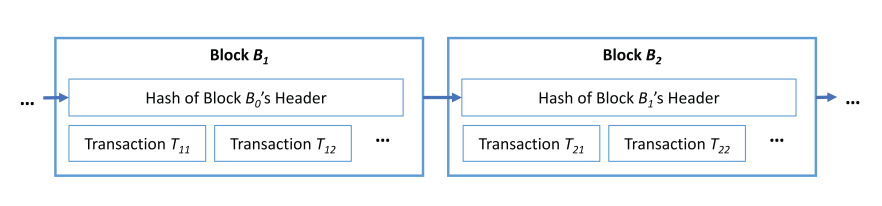
\includegraphics[width=\textwidth]{images/exemplo-de-blockchain.png}
    \caption{Estrutura básica de uma Blockchain}
    \label{fig:blockchain}
\end{figure}

Satoshi Nakamoto projetou a Blockchain do Bitcoin para atender as necessidade de uma moeda, contudo o protocolo extrapola essa finalidade, suportando operações mais complexas, além do simples escopo de um sistema de pagamentos.
Isto porque, ao invés de implementar uma lista preemptiva e exaustiva de todas as transações que pudessem vir a ser necessárias, o protocolo do Bitcoin imbui as transações com uma linguagem de script baseada em pilha, intencionalmente turing-incompleta, sem loopings ou recursividade, contendo algumas operações aritméticas, lógicas e criptográficas julgadas úteis para modelar as transações que a rede viria a suportar \cite{Narayanan2016a}.

As transações, unidades elementares da Blockchain, dependem dessa linguagem de script para definir o comportamento de suas entradas e saídas, duas listas que as compõem e indicam respectivamente de onde estão vindo os fundos e qual será a destinação deles.
Uma saída especifica uma quantidade em bitcoins e usa um script para 'trancar' este valor sob um desafio criptográfico, podendo ser utilizada por uma transação posterior que a referencie em uma de suas entradas.
Uma entrada contém uma referência à uma transação, especificamente para alguma de suas saídas que pretende utilizar, e o script que resolve o desafio relacionado àquela saída.
A checagem de uma transação se dá pela união dos scripts de entrada e saída e sua execução pelo cliente do Bitcoin, sendo considerada válida se, e somente se, para cada uma de suas entradas, a união do script com a respectiva saída de transação referenciada por ela resultar, ao fim do processo, em um valor verdade na pilha de execução do
interpretador\footnote{O artigo \cite{Bistarelli2019} ilustra em suas figuras o processo de execução de scripts passo-a-passo.}.

Diversos comportamentos foram então modelados, e o mais comumente utilizado entre eles implementa a operação que é o núcleo da rede Bitcoin - a transferência de moeda entre carteiras - implementada pelo script conhecido como P2PKH \emph{(Pay to Public Key Hash)}, que carrega um hash de uma chave pública e condiciona a utilização do valor na saída de uma transação à apresentação da chave pública que corresponda ao hash, juntamente com uma assinatura produzida pela chave privada da respectiva chave pública, permitindo que somente o detentor da chave privada possa utilizar o valor encaminhado a ele por meio da chave pública.
Outros scripts juntamente com este formam um pequeno conjunto de scripts creditados como seguros e alçados ao status de padrão no protocolo do Bitcoin.
Uma transação é considerada padrão quando só utiliza scripts padrões, e mais de 99,9\% das transações na Blockchain são padrões \cite{Bistarelli2019}.
A alta adesão não é coincidência, pois o cliente oficial do Bitcoin não permite a propagação de transações não-padrão pela
rede\footnote{Há outras verificações que impedem o recebimento e transmissão de uma transação na rede. Veja \url{https://en.bitcoin.it/wiki/Protocol_rules\#.22tx.22_messages}},
virtualmente negando o serviço a transações deste tipo, impondo ao seu proponente o ônus de propagar sua transação de forma externa à rede na tentativa de fazê-la alcançar os nós que tenham a eventual chance de incluir um bloco na Blockchain.

Essa linguagem de script demonstra a preocupação no projeto do Bitcoin para poder abarcar, caso fosse necessário, complexidades e regras de transação além do escopo de uma moeda ou pagamento.
Com ela torna-se possível projetar e realizar transações de garantia, vínculos contratuais, arbitragem privada e multi-assinaturas.
Mais ainda do que isso, no início de 2014 \cite{Greenspan2015} o protocolo passou a permitir a adição de até 80 bytes de metadados arbitrários em uma transação, abrindo o caminho, mesmo que limitado, para a utilização da blockchain como um \textbf{livro-razão distribuído} (em inglês \textbf{\textit{Distributed Ledger}}), uma fonte de dados onde seria possível registrar informações públicas, perenes e inalteráveis, acessíveis em qualquer lugar do mundo.
A \emph{Blockchain 2.0} surge para avançar o suporte ao conceito de livro-razão distribuído, trazendo novas tecnologias baseadas em blockchain, destacando-se entre elas as \emph{Smart Properties}, \emph{Smart Contracts} e \emph{DApps (Decentralized Applications)} \cite{Swan2015}.
Essas ferramentas elevam a expressividade e capacidade da Blockchain como uma plataforma para a criação de aplicações financeiras, semi-financeiras, e até mesmo aplicações com ativos que não são financeiros.

%% detalhamento do Bitcoin que o professor disse estar fora de escopo, sobre scripts no Bitcoin
% O Bitcoin permite à princípio scripts com tamanho de até 10 mil bytes e com dados de no máximo 520 bytes na pilha de execução\footnote{Informações retiradas do cliente oficial do Bitcoin, versão 0.19, no arquivo de cabeçalho referente a scripts, linhas {\color{RoyalBlue}\href{https://github.com/bitcoin/bitcoin/blob/0.19/src/script/script.h\#L23}{23}} e {\color{RoyalBlue}\href{https://github.com/bitcoin/bitcoin/blob/0.19/src/script/script.h\#L32}{32}}.}.

%% especificação do tipo de hashing que o Bitcoin faz. Não sei se no Ethereum é assim, então fica de fora do texto até que seja relevante
% Cada bloco tem uma referência única calculada a partir de seu conteúdo por meio de hashing\footnote{Especificamente, é realizado um hashing duplo utilizando SHA-256 nos campos que compõem o cabeçalho do bloco, representados em bytes \cite{bitcoinWikiHashing}.}

{\color{ForestGreen}Explicar que para criar o consenso, ou seja, escolher quem irá inserir o último bloco na cadeia, é necessário utilizar o mecanismo de consenso denominado Proof-of-Work (PoW). Explicar em que consiste o PoW. (2 parágrafos).}

\textbf{Fatos sobre a necessidade consenso}

\begin{itemize}
    \item A Blockchain pode ser centralizada ou distribuída, e pode ser permissionada ou pública.
    \item Uma Blockchain centralizada é operada por uma autoridade central ou um conjunto delas, que serão responsáveis que selecionar transações, montar blocos e adicioná-los.
    \item a Blockchain pública não contém barreiras de entrada para o sistema, e as criptomoedas todas operam nessa política de acesso. Blockchains permissionadas ou privadas surgiram para atender soluções comerciais e empresariais, podendo consistir em uma rede clientes de uma blockchain pública configurada para operar numa rede interna, ou utilizando blockchains com arquiteturas que considerem a permissão de uso, como o Hyperledger Fabric \cite{Indeterminado2019}.
    \item A Blockchain distribuída opera em uma base p2p e foi projetada sob a suposição da ausência de papéis de confiança aos integrantes da rede, o que implica em uma dificuldade óbvia de decidir quem será o responsável por incluir o próximo bloco.
    \item A Blockchain distribuída opera em uma arquitetura p2p e foi projetado para operar sem a confiança em usuários para realizar operações sensíveis e que poderiam destruir a rede em caso de uso mal intencionado. Sem haver um papel fixo para gerenciar a rede, decorre que o acesso a ela torna-se público e irrestrito e sem esse controle perde-se a proporção de nós na rede que sejam mal intencionados, não sendo possível derivar propriedades de segurança que tornariam mais simples o desenvolvimento do sistema.
    \item Devido à homogeneidade de papeis, a única saída é conferir a possibilidade de escrita a todos os participantes da rede, o que acarretaria em cada usuário escrevendo sua própria blockchain e realizando broadcast de sua versão aos demais levaria a múltiplas e incompatíveis versões na rede, destruindo sua funcionalidade. Para resolver essa questão é necessário estabelecer um consenso quanto às alterações na Blockchain e um período de tempo para que o consenso possa se propagar por toda a rede.
    \item O algoritmo de consenso organiza a escrita na blockchain em rodadas, estabelecendo um desafio computacional com uma dificuldade ajustada dinamicamente de acordo com a capacidade de processamento total da rede. Esse algoritmo estabelece que tem o direito de inserir um bloco na Blockchain o nó que apresentar um bloco válido (i.e., um bloco constituído somente por transações válidas) cujo cabeçalho contenha uma solução válida de acordo com a dificuldade pré-estabelecida no último bloco da rede.
    \item a participação no consenso é opcional, sendo possível configurar o software para somente obter os dados da Blockchain provindos da rede, e são denominados como \emph{light nodes}. Integrantes que participam do consenso e portanto tem uma chance de adicionar blocos são denominados \emph{mineradores}.
\end{itemize}

 \textbf{Sobre o Proof-of-Work}

\begin{itemize}
    \item O desafio computacional é baseado na ideia do HashCash \cite{Back2002} e foi denominado como \emph{Proof-of-Work} \emph{(PoW)}.
\end{itemize}
\subsection{Contratos inteligentes no Ethereum} \label{sub:sec:contratos-ethereum}

{\color{ForestGreen}Explicar para que servem e listar benefícios. (1 parágrafo).}

O conceito de \emph{Smart Contract} antecede o advento da blockchain, vislumbrando a possibilidade  de tornar um acordo formal (i.e. um contrato) firmado entre duas ou mais partes em um conjunto de regras computáveis que podem ser, portanto, embutidos no software ou hardware de propriedades com valor e que são controladas por meios digitais, com protocolos estabelecidos para que as partes possam interagir com as regras e desempenhar seus papéis.
Isso possibilita a execução automática do contrato sem a necessidade de intermediários, reduzindo a necessidade de confiança em terceiros e os custos de transação \cite{Bartoletti2019, Szabo1996}.
O Ethereum foi o primeiro e mais bem-sucedido projeto baseado em Blockchain voltado especificamente para a execução de Smart Contracts, fornecendo uma linguagem de programação turing-completa com suporte a funções criptográficas e de consulta de metadados da blockchain, permitindo expressar contratos na forma de programas que podem ser publicados na rede Ethereum e com os quais usuários e outros contratos podem interagir.

Invocações às funções de um contrato se dão por meio de uma transação contendo, entre outros parâmetros, os argumentos para a execução da função e um limite computacional compulsório a esta execução, expresso em termos de um recurso quantitativo denominado \emph{gas}.
O gas é a unidade fundamental do custo computacional na rede Ethereum, é convertido automaticamente a partir do \emph{Ether} --- a moeda base do Ethereum --- e a taxa de conversão é governada por uma equação definida no protocolo da plataforma, levando em conta estatísticas de uso da rede e ajustando o preço da computação de acordo com a demanda registrada na blockchain.
O usuário pode configurar na transação o quanto de gas deseja utilizar, desde que possua o respectivo saldo em Ether, até um limite máximo atribuído pelo próprio protocolo.
Essa mecânica incentiva um uso consciente da capacidade computacional da rede, contorna o problema da indecibilidade quanto ao fim ou não da execução de um programa, impedindo a parada da \emph{Ethereum Virtual Machine (EVM)} diante da execução de funções que, sem tal limitação, ao rodar indefinidamente ou por períodos extensos poderiam perturbar a taxa com que são processadas novas transações, e por fim serve para proteger os recursos do próprio usuário ao interagir com uma função de um Smart Contract cujo custo esteja além da expectativa, quer seja este custo inerente à função (devido à complexidade da operação) ou só produto de um código ineficiente ou mesmo incapaz de terminar.

{\color{ForestGreen}Explicar que a linguagem utilizada é denominada Solidity. Explicar o que é solidity. (1 parágrafo).}

A linguagem na qual Smart Contracts são publicados na rede Ethereum se chama \emph{Ethereum Virtual Machine code (EVM code)} --- uma linguagem de baixo nível baseada em pilhas, similar à linguagem \emph{Forth}.
Visando ampliar o acesso à tecnologia, a Fundação Ethereum desenvolveu também linguagens de programação de alto nível, com sintaxes similares às linguagens mais utilizadas no mercado, com compiladores para produzir EVM code a partir delas. O \emph{Solidity} é uma destas linguagens, com sintaxe similar a Java e C\texttt{++}, dispondo de um compilador com parâmetros configuráveis e um crescente ecossistema composto por padrões de desenvolvimento, bibliotecas e ferramentas de desenvolvimento\footnote{Para se inteirar do ecossistema Solidity, veja \href{https://github.com/bkrem/awesome-solidity}{https://github.com/bkrem/awesome-solidity} ou outras listas publicadas na internet. Entre as bibliotecas, destacam-se a \emph{\href{https://openzeppelin.com/}{OpenZeppelin}}, \emph{\href{https://github.com/dapphub/dappsys}{Dappsys}} e \emph{\href{https://github.com/modular-network/ethereum-libraries}{Modular Libraries}} por atualmente possuírem as maiores bases de usuários, segundo o site \emph{GitHub}.}, destacando-se o ambiente de desenvolvimento e implantação de Smart Contracts \emph{Remix}, utilizada para codificar, depurar e implantar os Smart Contracts do protótipo deste trabalho em redes de teste Ethereum.

{\color{ForestGreen}Explicar o código de um contrato simples que terá o atributo idPaciente, um map de urls de registros médicos e um método addUrl. (1 parágrafo). Explicar que esse contrato é escrito em um arquivo com extensão .sol}

Com Solidity é possível descrever tanto funções quanto estruturas de dados temporárias ou armazenadas na blockchain.
A coleção de dados armazenados na Blockchain compõe o que se denomina como estado da EVM. A Lista \ref{cod:exemploSmartContract} contém um exemplo de uso de Solidity, implementando um contrato que disponibiliza o acesso de resultado de exames a pacientes.

\lstset{basicstyle=\small, numbers=left, language=bash, keywordstyle=\color{blue}, numbersep=1pt, label={cod:exemploSmartContract}, caption={Exemplo de Contrato Inteligente}}
\begin{lstlisting}
 pragma solidity ^0.5.1;
 pragma experimental ABIEncoderV2;

 contract Hospital {

   enum CodigoResultado {negativo, positivo, inconclusivo, falha}

   struct Registro {
     int version;
     CodigoResultado resultado;
     string data;
     uint MinTime;
     uint MaxTime;
     string extHash;
   }

   mapping (string => Registro) registros;
   mapping (address => string[]) patientURLs;

   function addURL (address patient, string  memory url, Registro memory r) public;
   function getRegistro(string memory url) public view returns (Registro);
  }
\end{lstlisting}


{\color{ForestGreen}Explicar um exemplo passo-a-passo (Só TEXTO, Não Código) de um cliente que obtém o contrato do parágrafo anterior e o executa remotamente em uma máquina. (2 parágrafo).}

As funções implementadas no contrato apontam a existência de dois tipos de papeis relacionados, um que provê informações e outro que as consulta. O Smart Contract armazena duas tabelas, uma associando endereços a uma lista de URLs e outra associando um URL a um objeto do tipo Registro, que contém as informações de um exame. Essas tabelas são alimentadas por meio da função \emph{addURL} do contrato, sendo utilizada pelo Hospital que deseja disponibilizar os exames para consulta, e os exames podem ser consultados usando-se a função \emph{getRegistro}. Ambos os papeis necessitam possuir uma identidade na blockchain Ethereum, ou seja, possuir um endereço válido e ser capaz de publicar transações. Também é necessário possuir um cliente capaz de se conectar a rede para poder publicar novas transações. Já para a consulta de dados, é possível utilizar serviços Web de terceiros, como sites de visualização de transação, para resgatar uma atualização particular ou obter o estado atual das variáveis do contrato.

Este exemplo, embora introduza a sintaxe do Solidity, também incorre em três situações problemáticas que podem precisar de conserto. Primeiro, Smart Contracts tem seu código tornado público à rede no momento de sua implantação e suas funções podem ser utilizadas por qualquer usuário da rede. A ausência de controle no uso da função é um risco à integridade dos dados, uma vez que pode estar sujeita a alterações maliciosas. Um contrato deve impor uma política de acesso a funções sensíveis, implementando nestas funções verificações internas do endereço responsável pela interação, permitindo ou não a execução de acordo com tal política. Segundo, dados publicados na Blockchain são sempre públicos em sua visibilidade, embora possam ter diferentes escopos de acesso. Isso quer dizer que os dados relacionados aos exames serão públicos, expondo informações privativas a quem tiver acesso à Blockchain. Uma maneira de mitigar este problema e ainda assim manter a segurança da informação é publicar assinaturas dos dados, que não conterão informação sensível mas ainda servirão para verificar a integridade e imutabilidade dos dados armazenados externamente, na web. Terceiro, mesmo que não configurasse problema de privacidade, este uso da Blockchain tornaria o custo de operação muito alto, uma vez que a cada exame médico haveria um custo para armazenar múltiplas informações, sendo as mais caras as informações de tamanho dinâmico como a variável de texto \emph{data}. Embora o exemplo exemplifique uma estrutura de dados, na prática a Blockchain tem restrições computacionais de uso baseada no alto custo de armazenamento e processamento, o que significa que mesmo em um cenário onde não seja necessário a privacidade, ainda assim há um incentivo para esvaziar as estruturas de dados de informação relativa ao domínio de aplicação e ao invés disso utilizar ela somente como um meio para se verificar estes dados que estarão alocados em bases de dados externas à Blockchain.


% -------------------------------------------------------------------- %
\newpage
\section{Sistema Proposto}

\begin{itemize}
    \item {\color{red} Assuma nesta seção que os conceitos de blockchain, Ethereum, contratos inteligentes e criptografia baseada em atributos já foram definidos e explicados.}

    \item {\color{red}Cada parágrafo deve ter em torno de 10 linhas}

    \item {\color{red}Não mostrar código.}

\end{itemize}

\subsection{Visão Geral}
\label{sec:visaogeral}

{\color{ForestGreen}Explicar que o sistema é composto por X componentes (1 parágrafo).}

A arquitetura do protótipo é constituída por 5 módulos: um módulo Cliente, que é o maior módulo e que coordena o processamento de dados no sistema em conjunto com o módulo de Smart Contracts implantados na EVM.
O módulo cliente se conecta aos módulos DCPABE para as operações de criptografia no esquema ABE e Web3j para a conectividade com a Blockchain Ethereum e como interface de interação com os contratos.
Finalmente, um módulo servidor armazena e faz a distribuição de arquivos criptografados pelo cliente.

{\color{ForestGreen}Explicar a função de cada componente (1-2 parágrafos para cada um).}

O módulo do cliente é responsável por incorporar a camada lógica responsável por coordenar as atividades entre os demais componentes.

O módulo do servidor recebe, armazena e envia arquivos criptografados.
Presumiu-se que o servidor não fosse confiável, e por isso as informações nele estão sempre criptografadas.
Na implementação este módulo também armazenou, de forma temporária, chaves criptográficas que representam a posse de um atributo. Isso não é uma necessidade; tal função poderia ser transferida para qualquer serviço de transferência de arquivos, como um servidor dedicado sob controle do certificador, um serviço de hospedagem em nuvem ou mesmo por e-mail.

O módulo blockchain é responsável por armazenar de forma permanente e imutável o registro de documentos cifrados e a respectiva política de acesso ao documento, descrita em termos de uma forma booleana composta por funções lógicas E e OU com atributos como predicados.
A Blockchain utilizada para teste do protótipo durante o protótipo foi uma versão privada da rede Ethereum gerada e processada por um programa específico para este fim denominado como Ganache.

Também é necessário que a blockchain tenha a capacidade de executar smart contracts, e por isso a rede Bitcoin não foi escolhida para este trabalho.
Dentre as muitas opções de Blockchain que suportam Smart Contracts a rede Ethereum foi escolhida por ser o projeto mais popular e bem sucedido, considerando a base de usuários e também seu valor de mercado.

Em conjunção com a blockchain Ethereum, foi utilizado a biblioteca Web3j para conectar o cliente à rede privada.
O Web3j fornece a interface para a conexão por meio de socket a um provedor de dados da rede blockchain, que pode ser tanto uma rede local, um cliente Ethereum como o geth ou um serviço WEB como o Infura. Além disso, fornece implantação de contratos inteligentes, invocação de métodos destes contratos e classes geradas dinamicamente.

{\color{ForestGreen}Figura dos principais componentes em alto nível: programa cliente (exemplo celular ou notebook), servidor de armazenamento de arquivos; blockchain ethereum; contratos inteligentes; servidor de chaves de permissões.}

\begin{figure}[H]
  \centering
  \includesvg[width=1.1\linewidth]{images/diagrama-DCPABE.svg}
  \caption{Diagrama do sistema: (1) Geração de chaves privadas, públicas e pessoais de atributos, (2) aplicação de póliticas de acesso em massa em prontuários eletrônicos de pacientes (PEP), (3) Smart Contract de gestão de chaves públicas de atributos recebe novas chaves e as disponibiliza para consulta, (4) Smart Contract de gestão de arquivos cadastra novos arquivos relacionados a um usuário e permite a consulta de metadados que contém informações sobre o servidor em que os dados estão hospedados, (5) um servidor hospeda os dados criptografados, (6) o usuário pode consultar metadados sobre um arquivo, requisitá-lo ao servidor e descriptografar localmente, consultar novas chaves de atributos e atualizar tanto o conteúdo do documento quanto a política de acesso, comunicando a atualização aos Smart Contracts e servidores de arquivos. A linha tracejada indica uma conexão estabelecida em comum acordo entre as partes, podendo ser um canal seguro via web e }
  \label{fig:diagramaDCPABE}
\end{figure}

{\color{ForestGreen}Explicar um cenário de uso passo-a-passo (exemplo, milestone 1, mas com permissões direcionadas ao contexto de saúde, por exemplo um paciente quer dar permissão de acesso a médicos cardiologistas) (2 parágrafos)}.

O protótipo funcionaria então da seguinte forma: Uma paciente de nome Alice receberia um documento digital, tal como um encaminhamento ou exame, e precisa juntar ele ao seu prontuário médico. Ela utiliza o módulo cliente para criptografar o documento usando um esquema criptográfico ABE, cifrando o documento de acordo com uma política de acesso que ela tenha escolhido ou concordado em usar.
Para este caso de uso, suponhamos que a tal política seja "paciente OU (Hospital-X E Hematologista)".
Isso garante acesso ao próprio paciente e aos médicos daquela especialidade em um hospital específico, sem nunca remover o controle do nível de segurança das mãos do paciente e respeitando seu direito à informação.

Após aplicar criptografia ao documento, simultaneamente o cliente encaminha o documento para um servidor de arquivos e publica blockchain os parâmetros da cifra, referenciando um endereço válido informado informando juntamente com ela o nome do arquivo, o instante da transação e uma referência ao servidor onde o arquivo está armazenado.
Em um segundo momento Bob, o hematologista do Hospital X, ciente do agendamento da consulta de Alice com ele, usa o cliente para obter informações sobre que arquivos dela estão disponíveis na blockchain.
Ao baixar a descrição dos arquivos e verificar que a política de acesso é compatível com os atributos concedidos a ele enquanto usuário, e então ele requisita o documento cifrado ao servidor de arquivos e decifra o documento utilizando os parâmetros do Esquema ABE publicados na blockchain em conjunção com as chaves privadas pessoais referentes aos atributos que possui.

\subsection{Taxonomia de permissões}

{\color{ForestGreen}Explicar que o servidor de permissões deverá ser responsabilidade de uma organização apta para entregar as permissões online (ex. Ministério de Saúde ou algúm conselho federal/regional de medicina) (1 parágrafo)}.

As permissões de acesso a documentos se dão por meio da concessão de atributos a usuários feita por certificadores. O módulo cliente possui a capacidade para tornar qualquer usuário um certificador, que ficará registrado na blockchain a partir de seu endereço de carteira. Entidades como o Ministério da Saúde, os Conselhos Federais e Regionais de Medicina, e todos os laboratórios, clínicas e hospitais se tornariam certificadores, podendo emitir atributos utilizáveis na descrição de políticas de acesso para um prontuário médico. A identidade principal do certificador é seu endereço de carteira ao invés de sua razão social, que é acrescentada ao sistema somente para facilitar sua operação. Portanto, embora o sistema conceda a liberdade para que qualquer usuário torne-se um certificador, não seria possível forjar uma entidade previamente cadastrada a menos que o agente mal intencionado também tivesse posse da chave privada deste certificador.

{\color{ForestGreen}Explicar que a autenticação de uma pessoa para obter a permissão deverá ser realizada de forma externa ao sistema proposto (1 parágrafo).}

Atributos são gerados a partir de requisições feitas por usuários e publicadas na blockchain, por meio de um Smart Contract específico que armazena o estado destas requisições. É necessário que o usuário exista para realizar tal requisição, ou seja, é preciso que ele, anteriormente, tenha interagido com o contrato relativo à gestão de usuários, associando seus dados básicos pessoais a um endereço de carteira. Embora fosse possível criar um canal seguro usando criptografia elíptica para transmitir o arquivo com os atributos ao requisitante, isso estava além do escopo deste trabalho. Desta forma, uma vez geradas as chaves fica a critério do certificador escolher o método de envio, que pode depender ou não de sua infraestrutura de TI, ou pode requerer uma transmissão offline (presencial) dos arquivos que contém os atributos.

{\color{RoyalBlue} Cogitei no texto a entrega física de um arquivo do atributo mas o protótipo implementado sempre supõe que ele vai pegar o atributo de um servidor, não de um sistema de arquivos. Não sei se posso assumir essa redação ou se eu devo remover essa possibilidade do texto.}

{\color{ForestGreen}Explicar que foi realizada uma taxonomia das possíveis permissões que seriam utilizadas no sistema para o contexto médico. (3 parágrafos explicando como foi realizado o levantamento, me lembro que tinha um artigo e uma lista gigante que foi filtrada por quantidade de médicos).}

O sistema proposto pretende integrar diversas bases de dados de diferentes órgãos que, uma vez  certificadores, serão providos com a capacidade de publicar os atributos que forem necessários para a cifra dos documentos. A autonomia dos agentes para criar atributos levanta a necessidade de coordenação entre eles, de forma a manter políticas de acesso harmônicas e funcionais entre documentos que possam ser acessados por entidades distintas. Sem uma proposta de padronização, corre-se o risco das entidades desenvolverem padrões distintos e provavelmente conflitantes no que diz respeito ao escopo, à reutilização e à descrição textual de um atributo.

A diferença na hierarquia da estrutura das instituições na área da saúde, em suas competências e especialidades e suas políticas de acesso à informação podem resultar em diversas configurações distintas e incompatíveis quando descritos em um esquema criptográfico ABE. Um sistema que pretenda permitir o acesso a prontuários médicos distribuídos entre instituições com este esquema deve, portanto, propor também uma norma para a criação e gestão de atributos e de escrita das políticas de acesso . Para atingir este fim, buscou-se o denominador comum entre as exigências e restrições a que devem se condicionar todos os operadores na área da saúde, considerando-se o profissional da saúde como a unidade elementar desta análise , visto que uma política de atributos tem o potencial descritivo para modelar essas distintas responsabilidades.

O Código de Ética Médica (CEM) trata da conduta médica em diversos casos, incluindo também regras de conduta para o acesso à informações médicas, e proveu os elementos necessários para a elaboração de uma taxonomia de condição de acesso a estas informações, conforme mostra a figura 3.2.0 {\color{RoyalBlue}(vou referenciar)}. Isso já permite descrever qual será a política elementar e universal ao qual qualquer prontuário médico deve se submeter:

\[ CFM \vee CRM \vee Paciente \vee Terceiro\textnormal{-}Autorizado \]

Essa política padrão não impede a aplicação de outras políticas em subseções do prontuário, preservando informações de quem a princípio já possui acesso ao prontuário. Caso exista uma política de acesso em alguma subseção do prontuário, será necessário obrigatoriamente adicionar o acesso ao menos aos Conselhos de Medicina. Outras regras podem ser abstraídas a partir da taxonomia, como a necessidade de substituir a partícula $Paciente \vee Terceiro\textnormal{-}Autorizado$ por $Respons\acute{a}vel\textnormal{-}Legal$ caso o paciente seja menor de idade.

A escrita de política de acesso fica sujeita a uma normalização a partir da taxonomia apresentada, mas ainda é necessário adequar o escopo de atribuições dos funcionários de saúde entre os distintos órgãos em que podem trabalhar. A estratégia para propor uma taxonomia abrangente e relevante foi obter dados do DATASUS (Órgão que administra a consulta de informações do Sistema de Saúde Pública) sobre todas as profissões registradas no país na área da Saúde relativas ao início do ano de 2019. Na pesquisa obteve-se mais de 400 profissões distintas, que foram categorizadas pelo nível de ensino e agregadas pela área de atuação. Isso resultou em uma segunda taxonomia, disponível no Anexo I {\color{RoyalBlue}(referenciar)}, que serve como referência para a escrita de política de acesso usando termos e escopos comuns entre os certificadores. A entidade responsável por emitir o atributo a um médico seria o CRM de sua região. As entidades diversas emitiriam o restante dos atributos relativos às outras funções que necessitam acessar os dados do paciente, tais como setor administrativo ou o corpo de funcionários técnico-hospitalar.

{\color{ForestGreen}Figura da taxonomia}.

{\color{RoyalBlue}

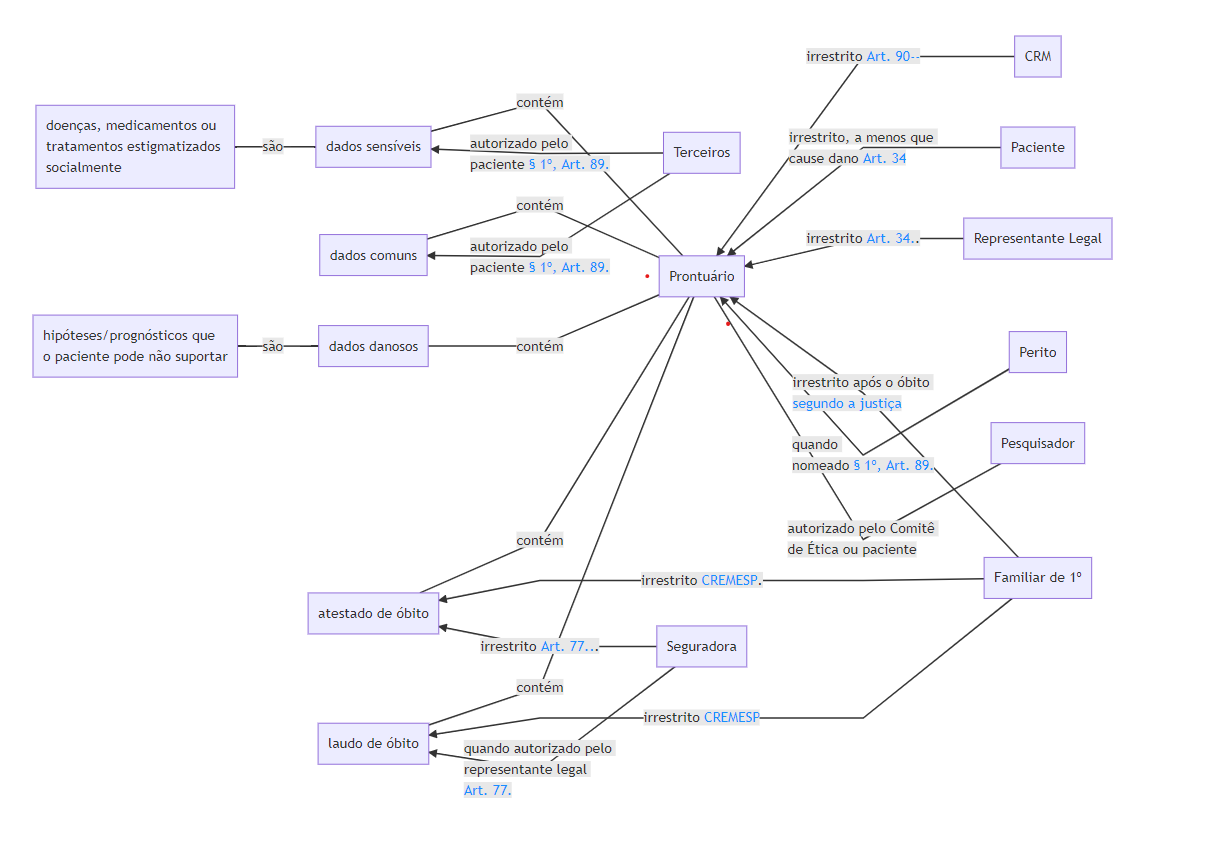
\includegraphics[width=\textwidth]{images/taxonomia-de-permissoes.png}

\href{https://mermaidjs.github.io/mermaid-live-editor/#/view/eyJjb2RlIjoiZ3JhcGggUkxcbkExW0NSTV0gLS0gaXJyZXN0cml0byA8YSBocmVmPVwiXCJodHRwOi8vYml0Lmx5L0PDs2RpZ2_DiXRpY2FNZWRpY2luYSNhcnQ5MFwiXCI-QXJ0LiA5MC0tPC9hPiAtLT4gIEJbUHJvbnR1w6FyaW9dXG5CIC0tLXxjb250w6ltfCBDW2RhZG9zIHNlbnPDrXZlaXNdXG5DIC0tLXxzw6NvfCBDMVtkb2Vuw6dhcywgbWVkaWNhbWVudG9zIG91IDxicj4gdHJhdGFtZW50b3MgZXN0aWdtYXRpemFkb3MgPGJyPiBzb2NpYWxtZW50ZV1cbkIgLS0tfGNvbnTDqW18IERbZGFkb3MgY29tdW5zXVxuQiAtLS18Y29udMOpbXwgRVtkYWRvcyBkYW5vc29zXVxuRSAtLS18c8Ojb3wgRTFbaGlww7N0ZXNlcy9wcm9nbsOzc3RpY29zIHF1ZSA8YnI-IG8gcGFjaWVudGUgcG9kZSBuw6NvIHN1cG9ydGFyXVxuQiAtLS18Y29udMOpbXwgRlthdGVzdGFkbyBkZSDDs2JpdG9dXG5CIC0tLXxjb250w6ltfCBHW2xhdWRvIGRlIMOzYml0b11cbkEyW1BhY2llbnRlXSAtLSBpcnJlc3RyaXRvLCBhIG1lbm9zIHF1ZSA8YnI-IGNhdXNlIGRhbm8gPGEgaHJlZj1cIlwiaHR0cDovL2JpdC5seS9Dw7NkaWdvw4l0aWNhTWVkaWNpbmEjYXJ0MzRcIlwiPkFydC4gMzQ8L2E-IC0tPiAgQltQcm9udHXDoXJpb11cbkEzW1JlcHJlc2VudGFudGUgTGVnYWxdIC0tIGlycmVzdHJpdG8gPGEgaHJlZj1cIlwiaHR0cDovL2JpdC5seS9Dw7NkaWdvw4l0aWNhTWVkaWNpbmEjYXJ0MzRcIlwiPkFydC4gMzQuPC9hPi4gLS0-ICBCW1Byb250dcOhcmlvXVxuQTRbRmFtaWxpYXIgZGUgMcK6XSAtLSBpcnJlc3RyaXRvIDxhIGhyZWY9XCJcImh0dHA6Ly9iaXQubHkvMlQ4NWhWTVwiXCI-Q1JFTUVTUDwvYT4uIC0tPiAgRlxuQTQgLS0gaXJyZXN0cml0byBhcMOzcyBvIMOzYml0byA8YnI-PGEgaHJlZj1cIlwiaHR0cHM6Ly9nbG8uYm8vMlQyTDRSaVwiXCI-c2VndW5kbyBhIGp1c3Rpw6dhPC9hPiAtLT4gIEJcbkE0IC0tIGlycmVzdHJpdG8gPGEgaHJlZj1cIlwiaHR0cDovL2JpdC5seS8yVDg1aFZNXCJcIj5DUkVNRVNQPC9hPiAtLT4gIEdcbkE1W1NlZ3VyYWRvcmFdIC0tIGlycmVzdHJpdG8gPGEgaHJlZj1cIlwiaHR0cDovL2JpdC5seS9Dw7NkaWdvw4l0aWNhTWVkaWNpbmEjYXJ0NzdcIlwiPkFydC4gNzcuLjwvYT4uIC0tPiAgRlxuQTUgLS0gIHF1YW5kbyBhdXRvcml6YWRvIHBlbG8gPGJyPiByZXByZXNlbnRhbnRlIGxlZ2FsIDxicj48YSBocmVmPVwiXCJodHRwOi8vYml0Lmx5L0PDs2RpZ2_DiXRpY2FNZWRpY2luYSNhcnQ3N1wiXCI-QXJ0LiA3Ny48L2E-IC0tPiAgR1xuQTZbUGVyaXRvXSAtLSBxdWFuZG8gPGJyPiBub21lYWRvIDxhIGhyZWY9XCJcImh0dHA6Ly9iaXQubHkvQ8OzZGlnb8OJdGljYU1lZGljaW5hI2FydDg5cDFcIlwiPiAmIzE2NyAxwrosIEFydC4gODkuPC9hPiAtLT4gQlxuQTdbUGVzcXVpc2Fkb3JdIC0tIGF1dG9yaXphZG8gcGVsbyBDb21pdMOqIDxicj4gZGUgw4l0aWNhIG91IHBhY2llbnRlIC0tLSBCXG5BOFtUZXJjZWlyb3NdIC0tIGF1dG9yaXphZG8gcGVsbyA8YnI-IHBhY2llbnRlIDxhIGhyZWY9XCJcImh0dHA6Ly9iaXQubHkvQ8OzZGlnb8OJdGljYU1lZGljaW5hI2FydDg5XCJcIj4gJiMxNjcgMcK6LCBBcnQuIDg5LjwvYT4gLS0-IENcbkE4W1RlcmNlaXJvc10gLS0gYXV0b3JpemFkbyBwZWxvIDxicj4gcGFjaWVudGUgPGEgaHJlZj1cIlwiaHR0cDovL2JpdC5seS9Dw7NkaWdvw4l0aWNhTWVkaWNpbmEjYXJ0ODlcIlwiPiAmIzE2NyAxwrosIEFydC4gODkuPC9hPiAtLT4gRCIsIm1lcm1haWQiOnsidGhlbWUiOiJkZWZhdWx0Iiwic2VjdXJpdHlMZXZlbCI6Imxvb3NlIn19}{Link do Diagrama (Ainda vou desenhar isso usando a biblioteca TikZ}

(quando eu refizer esse diagrama, vou incluir o MÉDICO. Esqueci do papel principal, mas já sei que ele tem acesso irrestrito se ele for o responsável pelo paciente)}

{\color{ForestGreen}Explicar que no sistema proposto existe um servidor de atributos ao qual se pedem as chaves públicas/privadas para realizar a encriptação/decriptação (1 parágrafo).}

Atributos são pares de chaves pública e um conjunto de chaves privadas pessoais que possibilitam a criptografia assimétrica. Um atributo precisa ser publicado na blockchain para ser utilizado pelos outros usuários, e considera-se publicado o atributo que tenha seus parâmetros de chave pública enviados ao Smart Contract que gerencia estas chaves. De posse da chave pública é possível criptografar um arquivo com uma política de acesso descrita em termos daqueles atributos e caso o usuário possua as respectivas chaves privadas pessoais também é possível descriptografar o conteúdo cifrado. As operações criptográficas sempre ocorrem localmente para evitar a exposição de informação sensível à rede a qual está conectado.

{\color{ForestGreen}Explicar como é realizado o passo-a-passo para o pedido/entrega das chaves (note que aqui a descrição é muito mais profunda que o que foi mencionado na visão geral) (1 parágrafo).}

O conjunto de chaves privadas pessoais deriva de uma chave privada secreta associada a um atributo público e de posse do certificador que a gerou. Para assegurar a unicidade da chave, também é necessário derivar a chave a partir de um identificador único (ID) associado ao usuário. Utilizar atributos com ID distintos impede a descriptografia de funcionar, assegurando que atributos não sejam intercambiáveis entre os usuários. {\color{RoyalBlue} existe um nome para esse problema onde alguém tentar ceder credenciais para alguém não autorizado. Usar aquela definição aqui}

O mecanismo de derivação de chaves privadas pessoais está atrelado ao processamento de requisições, impedindo o certificador de conceder chaves arbitrariamente, mas somente a partir de requisição prévia. Isso é uma estratégia para limitar o poder do certificador em criar atributos, e dessa forma abusar de sua autoridade para conceder acesso indevido a agentes não autorizados de forma. O certificador portanto consulta a blockchain para obter novas requisições e decide se irá processá-la ou não. Nos dois casos, a resposta retorna à blockchain assim que a chave é criada ou quando sua criação é negada, quer seja por decisão do certificação ou por falha devido a parâmetros incorretos.


\subsection{Contratos inteligentes com CBA}

Foram desenvolvidos cinco contratos inteligentes que permitem a autenticação, entrega de permissões e armazenamento de metadados dos prontuários eletrônicos dos pacientes. A seguir serão explicados cada um deles.

{\color{ForestGreen} Explicação do  SmartDCPABEAuthority (3 parágrafos). Ver abaixo os 3 parágrafos destrinchados.}

{\color{Magenta} 1 parágrafo para explicar o que faz o contrato (em linhas gerais).}

O contrato \emph{Authority} registra na Blockchain as entidades certificadoras disponíveis no sistema, tornando público seu endereço público na Ethereum, associando dados de identificação e a quantidade de atributos que a entidade já publicou.
o ID usado para derivar as chaves privadas dos atributos no esquema ABE é a chave privada que corresponde à chave pública do Ethereum.
Esse esquema permite que uma entidade possa ser identificável de forma única sem a necessidade de controle centralizada sobre o cadastro de novas unidades.
A escolha do ID visa impossibilitar um atacante de se passar pela entidade certificadora, uma vez que não há método computacionalmente viável para recuperar a chave privada de um endereço Ethereum a partir de uma chave pública.

{\color{Magenta} Inserir o código da linha 7 até 20.}

\lstset{basicstyle=\small, numbers=left, language=bash, keywordstyle=\color{blue}, numbersep=1pt, label={cod:SmartDCPABEAuthority}, caption={Dados em SmartDCPABEAuthority}}
\begin{lstlisting}
 contract SmartDCPABEAuthority is Collection {

 struct Certifier {
   address addr;
   bytes32 name;
   bytes32 email;
   uint64 numPublicKeys;
 }

 address[] public certifierAddresses;
 mapping (address => Certifier) certifiers;
\end{lstlisting}

{\color{Magenta} 1 parágrafo para explicar para que serve CADA UM dos structs, events e atributos. Exemplo. O struct X permite armazenar dados que servirão para Y. O atributo V armazena informações de W que servirão para Z.}

A struct Certifier armazena dados informações da autoridade responsável por publicar atributos e concedê-los a usuários. Além do endereço Ethereum, também é armazenado seu nome, e-mail e a quantidade de chaves que ele já publicou.
Tal unidade de controle é necessária porque as chaves são armazenadas em \emph{mappings}, conforme explicitado na Sessão \ref{sub:sec:contratos-ethereum}.

{\color{ForestGreen} Explicação do  SmartDCPABEKeys (3 parágrafos). Ver abaixo os 3 parágrafos destrinchados.}

{\color{Magenta} 1 parágrafo para explicar o que faz o contrato (em linhas gerais).}

O contrato \emph{Keys} disponibiliza a chave pública de atributos criados por autoridades.
Para fins de prototipagem foram implementadas somente as operação de inclusão e consulta de chaves, mas não de edição ou remoção. Seria trivial implementar isto no Smart Contract, mas não seria trivial e nem viável implementar os protocolos de revogação e substituição de atributos no módulo Cliente, responsável pelas operações criptográficas e pela coordenação das informações entre a Blockchain e o Servidor.

{\color{Magenta} Inserir o código da linha 6 até 24.}

\lstset{basicstyle=\small, numbers=left, language=bash, keywordstyle=\color{blue}, numbersep=1pt, label={cod:SmartDCPABEKeys}, caption={Dados em SmartDCPABEKeys}}
\begin{lstlisting}
 contract SmartDCPABEKeys is Collection {

 struct PublicKey {
  Bytes127 eg1g1ai;
  Bytes127 g1yi;
 }

 struct Bytes127 {
  bytes32 chunk1;
  bytes32 chunk2;
  bytes32 chunk3;
  bytes31 chunk4;
  uint8 lastChunkSize;
 }

 mapping (address => bytes32[]) publicKeyNames;
 mapping (address => mapping (bytes32 => PublicKey)) ABEKeys;
\end{lstlisting}

{\color{Magenta} 1 parágrafo para explicar para que serve CADA UM dos structs, events e atributos.}

a estrutura \emph{Bytes127} foi criada como um container econômico para armazenar os elementos gerados pela biblioteca jPBC \emph{(Java Pairing-Based Cryptography)} \cite{DeCaro2011}.
O tamanho dos elementos varia entre 120 a 124 bytes de informação e, embora o Solidity disponha da estrutura de dados \emph{bytes} para armazenar bytes em tamanho arbitrário, seu custo é maior.
Dados consomem gas, e quando são utilizadas estruturas de dados de tamanho dinâmico, o valor é maior do que suas contrapartes estáticas, justificando a criação de uma estrutura que divida os dados em um conjunto de elementos de tamanho fixo.
A estrutura \emph{PublicKey} armazena a chave pública gerada pela biblioteca \emph{DCPABE}\footnote{código fonte: \href{https://github.com/stefano81/dcpabe}{\texttt{https://github.com/stefano81/dcpabe}}. Para uma análise teórica, ver \cite{Lewko2011}}, que são representadas por duas sequências de bytes como mostra o código.
O mapa \emph{publicKeyNames} mapeia um endereço de uma autoridade a uma lista de nomes de atributos representados como bytes.
O mapa \emph{ABEKeys} contém, para cada endereço cadastrado, um submapa relacionando o nome do atributo representado em bytes com uma chave pública.

{\color{ForestGreen} Explicação do  SmartDCPABEFiles  (3 parágrafos). Ver abaixo os 3 parágrafos destrinchados.}

{\color{Magenta} 1 parágrafo para explicar o que faz o contrato (em linhas gerais).}

O contrato \emph{Files} mantém disponível na blockchain informações sobre a hospedagem do arquivo de prontuários e também os dados do objeto \emph{Ciphertext} produzido pela Biblioteca DCPABE, necessário para realizar a descriptografia. O contrato também gerencia informações sobre as bases de dados onde os arquivos estão hospedados.

{\color{Magenta} Inserir o código da linha 6 até 39.}

\lstset{basicstyle=\small, numbers=left, language=bash, keywordstyle=\color{blue}, numbersep=1pt, label={cod:SmartDCPABEFiles}, caption={Dados em SmartDCPABEFiles}}
\begin{lstlisting}
 contract SmartDCPABEFiles is Collection {

 struct Recording {
  uint64 serverID;
  bytes32 key;
  bytes32 hashing;
  uint64 timestamp;
 }

 struct Ciphertext {
  string policy;
  bytes c0;
  bytes c1;
  bytes c2;
  bytes c3;
 }

 struct FileServer {
  bytes32 domain;
  bytes32 path;
  uint16 port;
 }

 uint64 public numServers;
 mapping (address => string[]) fileNames;
 mapping (address => mapping(string => Recording)) files;
 mapping (address => mapping(string => Ciphertext)) ciphertexts;

 FileServer[] servers;
\end{lstlisting}

{\color{Magenta} 1 parágrafo para explicar para que serve CADA UM dos structs, events e atributos.}

A Estrutura \emph{Recording} informa a base de dados na qual o arquivo está hospedado e qual é a sua identificação no servidor, o hashing para permitir a verificação de integridade e uma marca temporal para manter registro público do momento de sua publicação na Blockchain. Seria possível remover o campo timestamp e trabalhar somente com altura ou timestamp do bloco em que a transação foi validada, economizando o uso de gas, porém deixando de possuir uma data exata de publicação de um documento. A estrutura \emph{Ciphertext} contém a política de acesso utilizada para cifrar o arquivo e um conjunto de parâmetros (c0 a c3) que resultam do processo de criptografia e que são necessários para decifrar o documento. A estrutura \emph{FileServer} contém informações para conexão com uma base de dados na Internet. O contrato mantém uma lista de servidores \emph{servers} e um par de mapas \emph{files} e \emph{ciphertexts} com estrutura similar, ligando endereços de usuários a submapas que associam, por sua vez, um nome de arquivo às estruturas de dados \emph{Recording} e \emph{Ciphetext} relacionadas àquele arquivo. Disso segue-se que uma edição no conteúdo é mais barato que a alteração no nome do documento, uma vez que no caso do conteúdo somente o hashing e o timestamp são atualizados, enquanto que na renomeação o mapa armazena o arquivo como se fosse um novo, sendo necessário publicar os dados do arquivo e deletar aqueles que estavam disponibilizados.

{\color{ForestGreen} Explicação do  SmartDCPABERequests  (3 parágrafos). Ver abaixo os 3 parágrafos destrinchados.}

{\color{Magenta} 1 parágrafo para explicar o que faz o contrato (em linhas gerais).}

O contrato \emph{Requests} é responsável por lidar com requisições de concessão de atributos.
Usuários do sistema publicam suas requisições e as autoridades certificadoras podem checar por requisições pendentes e atendê-las ou rejeitá-las.
Uma requisição pode solicitar a concessão de um ou mais atributos a um mesmo certificador e é consumida quando processada, não sendo possível alterar novamente seu status.
A transmissão dos atributos ocorre fora da blockchain e pode usar qualquer meio de comunicação considerado seguro entre as partes.

{\color{Magenta} Inserir o código da linha 6 até 35.}

\lstset{basicstyle=\small, numbers=left, language=bash, keywordstyle=\color{blue}, numbersep=1pt, label={cod:SmartDCPABERequests}, caption={Dados em SmartDCPABERequests}}
\begin{lstlisting}
 contract SmartDCPABERequests is Collection {

 enum KeyRequestStatus {
  PENDING,
  OK,
  REJECTED
 }

 struct KeyRequest {
  KeyRequestStatus status;
  uint64 timestamp;
  uint64 responseTimestamp;
  bytes32[] attrNames;
 }

 event pendingRequestIndexChanged(uint64 oldIndex, uint64 newIndex);
 event pendingRequesterIndexChanged(uint64 oldIndex, uint64 newIndex);

 mapping (address => address[]) pendingRequesters;
 mapping (address => mapping (address => uint64[]))  pendingRequests;
 mapping (address => mapping (address => KeyRequest[]))  requests;
\end{lstlisting}

{\color{Magenta} 1 parágrafo para explicar para que serve CADA UM dos structs, events e atributos.}

A estrutura \emph{KeyRequest} representa uma requisição de atributos, contendo um campo para indicar a situação, marcas temporais da criação e processamento da requisição e uma lista de nomes de atributos representados como sequências de 32 bytes (Bytes32).
As situações estão listadas no enum \emph{KeyRequestStatus}, e podem ser expandidas para um conjunto maior de situações, conforme a necessidade das entidades que utilizem um sistema assim.
Dois eventos notificam sobre o processamento de requisições, para que os interessados possam atualizar seu cache local com a blockchain e obter assim o estado mais atualizado das requisições.
O mapa \emph{requests} usa endereços de certificadores como chave primária para submapas cujas chaves são os endereços de usuários e que levam às listas de requisições feitas por eles.
O mapa \emph{pendingRequests} segue esta mesma estrutura, com a diferença de apenas armazenar os índices das listas de requisições em \emph{requests} que estão pendentes de processamento.
O mapa \emph{pendingRequesters} mantém os endereços de usuários com requisições pendentes em listas agregadas por certificador, possibilitando que estes possam iterar pelo mapa \emph{pendingRequests}, obtendo os índices de acesso das requisições de interesse gravadas em \emph{requests}.

{\color{ForestGreen} Explicação do  SmartDCPABEUsers  (3 parágrafos). Ver abaixo os 3 parágrafos destrinchados.}

{\color{Magenta} 1 parágrafo para explicar o que faz o contrato (em linhas gerais).}

O contrato \emph{Users} gerencia o cadastro de usuários passíveis de obter atributos no esquema de criptografia ABE e exercer papeis dentro do deste sistema, implementando funções básicas de inclusão, consulta e checagem de usuários válidos.
A estrutura \emph{User} atrela dados básicos de identificação a um endereço válido de carteira Ethereum, e instâncias desta estrutura são salvas em um mapa \emph{users}, onde a chave deste mapa é o próprio endereço do usuário.
A lista \emph{userAddresses} armazena todos os endereços já cadastrados para permitir a iteração, se necessária, sobre as chaves do mapa \emph{users}.

{\color{Magenta} Inserir o código da linha 6 até 16.}

\lstset{basicstyle=\small, numbers=left, language=bash, keywordstyle=\color{blue}, numbersep=1pt, label={cod:SmartDCPABEUsers}, caption={Dados em SmartDCPABEUsers}}
\begin{lstlisting}
 contract SmartDCPABEUsers is Collection {

 struct User {
  address addr;
  bytes32 name;
  bytes32 email;
 }

 address[] public userAddresses;
 mapping (address => User) users;
 uint64 public numUsers;
\end{lstlisting}

{\color{Magenta} 1 parágrafo para explicar para que serve CADA UM dos structs, events e atributos.}

{\color{RoyalBlue} esse parágrafo foi agregado ao anterior porque os dois são pequenos, afinal o código deste contrato é pequeno.}

\subsection{Arquitetura Blockchain}

Como mencionado na Seção \ref{sec:visaogeral}, o sistema é composto por 3 componentes: cliente, servidor, e a Blockchain. A Figura X mostra o relacionamento entre esses componentes.

{\color{ForestGreen} Fazer uma figura simples que mostre os 3 componentes interligados. }


{\color{ForestGreen} Explicar implementação do cliente (5 parágrafos). Ver abaixo os 5 parágrafos destrinchados. }

{\color{Magenta} 1 parágrafo para explicar que para realizar a conexão com a Blockchain usou o web3j (explique em 2-3 linhas o web3j).}

A Web3j fornece conectividade com diferentes fontes de dados para consulta do estado de transações e envio de novas transações em blockchains compatíveis com o protocolo JSON-RPC Ethereum\footnote{ver \href{https://github.com/ethereum/wiki/wiki/JSON-RPC}{https://github.com/ethereum/wiki/wiki/JSON-RPC}.}, compreendendo a rede principal (\emph{MainNet}), as redes de teste oficiais Ropsten, Rinkeby e Kovan, redes permissionadas usando o Hyperledger Besu ou simulações da rede Ethereum para teste por meio de programas como o Ganache.
A Web3j se conecta ao provedor de dados por meio de Protocolos HTTP/HTTPS e IPC.

\lstset{basicstyle=\small, numbers=left, language=java, keywordstyle=\color{blue}, numbersep=1pt, label={cod:conexãoBlockchain}, caption={Código para conexão com a Blockchain usando o web3j}}

\begin{lstlisting}
 private final Web3j web3j;

 public BlockchainConnection(String networkURL, ...) {
   // codigo omitido por brevidade
   web3j = Web3j.build(new HttpService(networkURL));
 }
\end{lstlisting}

{\color{Magenta} 1 parágrafo para explicar as 3 linhas mais importantes do código fonte de como realizar a conexão. Explicar cada linha do código. }

Dentro do módulo Cliente, a classe \emph{BlockchainConnection} é a responsável por lidar com a Blockchain por meio do Web3j e as classes em Java que representam os Smart Contracts, e exige somente um endereço de rede válido para uma porta no computador ou rede local onde exista comunicação com um programa compatível com a API JSON-RPC do Ethereum, ou para um serviço Web na internet que ofereça a API, tais como os sites Infura e Ethercluster.
O endereço informado é armazenado no cache do programa para uso em execuções futuras.

{\color{Magenta} 1 parágrafo para explicar que para encriptar um documento utilizando atributos usou a dcpabe.}

A biblioteca DCPABE desenvolvida em Java possui suporte à operações criptográficas do protocolo ABE em um ambiente com múltiplas autoridades, conforme descrito em \cite{Lewko2011}.
Ela depende por sua vez da biblioteca \emph{jPBC} (Java Pairing Based Cryptography), a primeira e mais abrangente biblioteca de código aberto para criptografia baseada em emparelhamento em Java e compatível com Android, tendo o objetivo explícito de portar a biblioteca PGC\footnote{mais informações em \href{https://crypto.stanford.edu/pbc/}{https://crypto.stanford.edu/pbc/}}, originalmente escrita em C, para código nativo em Java e oferecer uma interface para essa biblioteca \cite{DeCaro2011}.
A DCPABE fornece todo o ferramentário necessário para o uso do esquema ABE, incluindo a geração de parâmetros globais, geração de chaves privadas, públicas e pessoais dos atributos, cifra e deciframento de fluxos de dados.
Ao criptografar um documento, um objeto do tipo \emph{Ciphertext} contendo os parâmetros necessários para a decifragem é serializado e escrito no início do arquivo container dos bytes criptografados.
Esse comportamento foi alterado para produzir um artefato equivalente, serializável em JSON, escrito em um arquivo separado daquele que contem os bytes criptografados, com a finalidade de poder publicar na Blockchain somente este artefato JSON, ao invés de todo o arquivo, e assim reduzir os custos de transação e viabilizar o uso da rede Ethereum.

{\color{Magenta} 1 parágrafo para explicar as 3 linhas mais importantes do código fonte de como realizar a encriptação. Explicar cada linha do código.}

\lstset{basicstyle=\small, numbers=left, language=java, keywordstyle=\color{blue}, numbersep=1pt, label={cod:métodoCriptografia}, caption={Criptografando um arquivo usando a biblioteca DCPABE}}

\begin{lstlisting}
 public void encrypt(String file, String policy, String[] authorities) {
   // codigo omitido por brevidade
   AccessStructure as = AccessStructure.buildFromPolicy(policy);
   Message m = DCPABE.generateRandomMessage(gp);
   CiphertextJSON ct = new CiphertextJSON(DCPABE.encrypt(m, as, gp, pks));
   r = new Recording(path, file, ct);
   r.encryptFile(m);
 }
\end{lstlisting}

% O objeto \emph{as}, instância da classe \emph{AccessStructure}, armazena uma representação matricial da fórmula boooleana descrita em \emph{policy}, produzindo uma estrutura de acesso de um \emph{LSSS} (Linear Secret Sharing Scheme), tornando a fórmula um elemento matricial vetorial compatível com a estrutura matemática necessária ao funcionamento dos algoritmos definidos pelo DCPABE.

A classe \emph{Client} implementa a função \emph{encrypt}, em parte exposto seção de código \ref{cod:métodoCriptografia}.
A função encrypt exige os parâmetros \emph{file} contendo o nome do arquivo a ser criptografado, \emph{policy} contendo uma política de acesso e o vetor \emph{authorities} contendo o ID das autoridades dos atributos relacionados em \emph{policy}.
Na linha 3 o objeto \emph{as}, instância da classe \emph{AccessStructure}, armazena uma representação matricial gerada a partir da fórmula boooleana descrita em \emph{policy}, tornando a fórmula em um elemento matricial vetorial compatível com a estrutura matemática necessária ao funcionamento dos algoritmos definidos pelo DCPABE.
Na linha 4 é definido como mensagem \emph{m} um elemento aleatório pertencente ao grupo do aparelhamento definido pelos parâmetros globais \emph{gp} -- o mesmo utilizado para a geração de chaves privas dos atributos.

Na linha 5 a mensagem m é ocultada sob a criptografia ABE utilizando a matriz \emph{as}, a mensagem \emph{m}, os parâmetros globais \emph{gp} e um vetor \emph{pks} com as chaves públicas de todos os atributos mencionados em \emph{policy}, retornando uma instância equivalente à da classe \emph{Ciphertext}, com a capacidade de ser serializada em JSON, e na linha 7 o arquivo é cifrado usando um algoritmo AES\footnote{Especificamente, é usada a classe AESEngine da biblioteca Bouncy Castle com configuração padrão. Ver \href{https://people.eecs.berkeley.edu/~jonah/bc/org/bouncycastle/crypto/engines/AESEngine.html}{https://people.eecs.berkeley.edu/~jonah/bc/org/bouncycastle/crypto/engines/AESEngine.html}} e a mensagem \emph{m} como chave. A descriptografia consiste em fornecer as chaves pessoais dos mesmos atributos usados na criptografia, aplicando o esquema ABE para obter a mensagem \emph{m} e usando-a como chave do algoritmo AES para descriptografar o conteúdo desejado.

{\color{Magenta} 1 parágrafo para explicar as 3 linhas mais importantes do código fonte de como acessar um contrato inteligente. Explicar cada linha do código.}

\lstset{basicstyle=\small, numbers=left, language=java, keywordstyle=\color{blue}, numbersep=1pt, label={cod:acessoSmartContract}, caption={Acessando um Smart Contract na Blockchain}}

\begin{lstlisting}
 private CiphertextJSON getCiphertext(String user, String fileName) {
   Tuple5<String, byte[], byte[], byte[], byte[]> ciphertextData;
   try {
     ciphertextData = contractFiles.getCiphertext(user, fileName).send();
     if (!ciphertextData.getValue1().equals("")) {
       // codigo usando os dados retornados pelo contrato
     }
   } catch (Exception e) { ... }
 }
\end{lstlisting}

O Acesso aos Smart Contracts em Java é intermediado por classes "wrappers", isto é, classes geradas automaticamente a partir do EVM Code e da ABI \emph{(Application Binary Interface)} de Smart Contracts para interação com o contrato.
Estas classes contém métodos que correspondem às funções nos Smart Contract, possuindo dois métodos a mais, um para implantar o contrato na EVM e outro para carregar o contrato, caso já tenha sido implantado.
Uma vez inicializado, a interação ocorre como exemplifica a sessão de código \ref{cod:acessoSmartContract}.
Na linha 4 o método \emph{getCiphertext} do objeto \emph{contractFiles}, wrapper do contrato \emph{SmartDCPABEFiles}, recebe os argumentos necessários à função, prepara um objeto que representa uma chamada remota ao contrato, que é enviada à rede Ethereum por meio da invocação do método \emph{send()} ao fim da linha.

Funções de Smart Contracts podem retornar dados, e se for o caso, serão inseridos em um objeto do tipo \emph{TupleN}, sendo N o número de parâmetros retornados. Este objeto possui métodos na forma \emph{getValueN()} para acessar o n-ésimo valor de retorno do Smart Contract.
A checagem feita na linha 5 é necessária para identificar se o objeto retornado pelo Smart Contract é vazio.
Isto é necessário porque a implementação da EVM não possui um elemento nulo como na maioria das linguagens mais populares, e também não suspende a execução e retorna um erro quando tenta-se acessar uma chave inexistente de um mapa.
Quando a EVM encontra uma variável indefinida ou inexistente, seu comportamento padrão é retornar um valor do mesmo tipo da variável que corresponda ao valor FALSO de uma variável booleana.
Sem um mecanismo de erro ou identificação de valores nulos, torna-se necessário checar o valor de alguma das variáveis recebidas cujo valor não possa ser equivalente ao FALSO booleano.
No código \ref{cod:acessoSmartContract}, a variável escolhida é \emph{policy}, que ocupa a posição 1 da tupla e que nunca pode ser igual a uma string vazia, visto que isto significaria que o conteúdo não está criptografado, necessariamente significando que o valor de retorno se refere a valores nulos ou inexistentes.
Confirmado que os dados recebidos realmente existem, estes são processados conforme a necessidade, no escopo aninhado à verificação, na linha 6.

{\color{ForestGreen} Explicar implementação do servidor (3 parágrafos). Ver abaixo os 3 parágrafos destrinchados. }

{\color{Magenta} 1 parágrafo para explicar que o servidor utiliza REST para prover os serviços via web  (explique em 2-3 o que é REST).}

O módulo do servidor conta com uma estrutura padrão de acordo com os princípios REST, ou seja, oferece uma API acessível (via protocolo HTTP) com métodos GET, POST e PUT, atribui URIs a todos os recursos sob gestão do servidor e possui um modelo de comunicação \emph{stateless}, i.e., toda a informação necessária à interação deve estar contida na mensagem recebida pelo servidor, sem a necessidade dele controlar o estado de comunicação ou contexto da interação de cada um dos clientes \cite{Mark2013}.
O método DELETE não é implementado porque o sistema proposto é contextualizado e modelado para manter o registro permanecente e inviolável de dados de pacientes médicos, não havendo justificativa para a exclusão dos dados, uma vez que o sigilo é preservado e operações de atualização de dados são permitidas nos cenários onde for preciso atualizar ou corrigir os dados armazenados.
O módulo cliente utiliza a classe \emph{ServerConnection} para encapsular o acesso ao servidor, que foi executado localmente durante todas as fases de desenvolvimento e experimentação do protótipo.

{\color{Magenta} 1 parágrafo para explicar que o servidor possui o serviço para inserir um documento e para recuperar um documento.}

a API disponível permite o envio, substituição e recuperação de arquivos enviados ao servidor.
As URIs dos arquivos no servidor são construídas a partir de hashes SHA-256 gerados aleatoriamente, sendo gerados e enviados ao cliente como resposta de uma requisição sinalizando o envio de um novo arquivo para o servidor.
Sendo exigido para a publicação na Blockchain, o cliente precisa informar este hash que passa a ser tratado como uma chave de acesso para o arquivo no servidor, junto com a identificação do servidor e outros dados, conforme as estruturas de dados definidas no contrato SmartDCPABEFiles exigem (ver código \ref{cod:SmartDCPABEFiles}).
Usuários do sistema interessados no arquivo acessam seus metadados na Blockchain, entre eles a identificação do servidor e a chave que compõe a URI.
A partir daí o cliente pode montar a URL da requisição do arquivo e obtê-lo do servidor.

{\color{Magenta} 1 parágrafo para explicar que o servidor insere e recupera os prontuários eletrônicos de pacientes diretamente do seu sistema de arquivos advindos das requisições web.}

O servidor foi implementado para salvar os arquivos diretamente em seu sistema de arquivos local, sem criptografia adicional sobre o conteúdo uma vez que este já é enviado criptografado pelo cliente, restringindo acessos não autorizados por terceiros.
O fato do arquivo ser entregue sempre que requisitado a princípio não apresenta violações à privacidade e segurança dos dados, uma vez que está criptografado e só poderá ser decifrado por quem possua os atributos compatíveis com a política de acesso, porém é possível que um atacante escolha acumular arquivos sob sua posse e aguardar pela descoberta de vulnerabilidades críticas nas bibliotecas de criptografia que possibilitariam, no pior cenário possível, a quebra da criptografia. A fim de evitar isso, pode-se acrescentar desafios criptográficos que provem que o requisitante realmente possui os atributos necessários para decifrar o arquivo.

Pode-se recorrer a um esquema baseado no conceito da Prova de Conhecimento-Zero \emph{(Zero Knowledge-Proof - ZPK)}, onde um verificador (o servidor) pode ser "convencido" que um provador (o cliente) realmente possui um segredo, sem com isso ter de expor alguma informação que altere o nível de conhecimento prévio do verificador sobre aquele segredo \cite{Rice2010,Buchanan2017}.
Considere que o servidor deva se convencer da legitimidade da aquisição\footnote{interpretando uma aquisição legítima como aquela em que de fato o cliente possui a capacidade de descriptografar o conteúdo solicitado.} de um arquivo por um usuário, sem que o usuário tenha que revelar suas chaves ou sua identidade, evitando neste último caso o ônus ao servidor de verificar na Blockchain o histórico de concessões de atributos àquela identidade e testar a compatibilidade deles com a política de acesso do arquivo em questão, introduzindo estados intermediários e mutáveis entre requisições do cliente devido à consulta na Blockchain, que implicarão na quebra do princípio REST da comunicação sem estados.

Uma solução viável é exigir ao cliente que, no ato do envio de um arquivo para ser hospedado, calcule o hashing deste arquivo, cifre este valor com a mesma política de acesso usada para o arquivo e então envie este par de arquivos cifrados ao servidor.
O comportamento do servidor seria levemente modificado para que, diante de uma requisição de um arquivo sem parâmetros adicionais, a resposta seria o objeto cifrado que contém o valor do hashing enviado anteriormente pelo cliente.
Um usuário com as credenciais necessárias seria capaz de decifrar esse objeto, realizando novamente a requisição do mesmo arquivo, desta vez informando o hashing como parâmetro.
Diante de uma requisição de arquivo com algum parâmetro adicionado, o servidor verifica se seu valor é equivalente ao valor do hashing do arquivo sob sua posse.
Seria impraticável tentar acertar o valor do hashing ao acaso, de forma que caso sejam equivalentes, torna-se evidente que o usuário tem consigo os atributos necessários para decifrar o conteúdo do arquivo e o servidor envia o arquivo, negando o acesso nos casos contrários.

{\color{ForestGreen} Explicar implementação da Blockchain (4 parágrafos). Ver abaixo os 4 parágrafos destrinchados. }

{\color{Magenta} 1 parágrafo para explicar que a Blockchain utilizada foi a testnet (explicar que existe a main e a testnet, onde a testnet é utilizada por desenvolvedores serve para realizar implantações de teste sem dispender recursos financeiros.}

{\color{Magenta} 1 parágrafo para explicar que a rede Blockchain foi implantada em um computador usando o Ganache. Explicar o que é o ganache e o que entrega a implantação (X mineradores? X full nodes, etc).}

{\color{Magenta} 1 parágrafo para explicar que a Blockchain possui 5 contratos inteligentes mencionados na Seção anterior.}

{\color{Magenta} 1 parágrafo para explicar que a implantação dos contratos inteligentes usou o Metamask. Explicar o que é o Metamask e o que especificamente você usou dele: ver identificadores das transações, conversão de .sol para .abi. Explicar o que é .abi.}

% -------------------------------------------------------------------- %
\newpage
\section{Trabalhos Relacionados}

\subsection{Sistemas de saúde com Blockchain e CBA}

\subsection{Sistemas de saúde com CBA}
\label{sub:sec:saude-cba}

\subsection{Sistemas gerais com CBA}

Caso não hajam trabalhos na seção~\ref{sub:sec:saude-cba}.

% -------------------------------------------------------------------- %
\newpage
\section{Resultados Experimentais}



% -------------------------------------------------------------------- %
\newpage
\section{Conclusões e Trabalhos futuros}

\begin{itemize}
  \item gasto financeiro
  \item problema energético
  \item sugestão: hyperledger Fabric / hyperledger Besu.
  \item implementar ZPK no servidor
\end{itemize}

\bibliography{doc}
\bibliographystyle{plainnat}

% -------------------------------------------------------------------- %
\newpage
\section{Anexo I}

PESSOAL DE SAÚDE - NÍVEL SUPERIOR
\begin{enumerate}
    \item ANESTESISTA
    \item ASSISTENTE SOCIAL
    \item BIOQUÍMICO/FARMACÊUTICO
    \item CIRURGIÃO GERAL
    \item CLÍNICO GERAL
    \item ENFERMEIRO
    \item FISIOTERAPEUTA
    \item FONOAUDIÓLOGO
    \item GINECO OBSTETRA
    \item MÉDICO DE FAMÍLIA
    \item NUTRICIONISTA
    \item ODONTÓLOGO
    \item PEDIATRA
    \item PSICÓLOGO
    \item PSIQUIATRA
    \item RADIOLOGISTA
    \item SANITARISTA
    \item OUTRAS ESPECIALIDADES MÉDICAS
    \item OUTRAS OCUPAÇÕES DE NÍVEL SUPERIOR RELACIONADOS À SAÚDE
\end{enumerate}
PESSOAL DE SAÚDE - NÍVEL TÉCNICO TÉCNICO/AUXILIAR
\begin{enumerate}
    \item AUXILIAR DE ENFERMAGEM
    \item FISCAL SANITÁRIO
    \item TÉCNICO DE ENFERMAGEM
    \item TÉCNICO E AUXILIAR DE FARMÁCIA
    \item TÉCNICO E AUXILIAR DE LABORATÓRIO
    \item TÉCNICO E AUXILIAR EM NUTRIÇÃO E DIETÉTICA
    \item TÉCNICO E AUXILIAR EM FISIOTERAPIA E REABILITAÇÃO
    \item TÉCNICO E AUXILIAR EM SAÚDE ORAL
    \item TÉCNICO E AUXILIAR EM VIG SANITÁRIA E AMBIENTAL
    \item TÉCNICO E AUXILIAR EM EQUIP MÉDICO-HOSPITALARES
    \item TÉCNICO E AUXILIAR EM RADIOLOGIA MÉDICA
    \item TÉCNICO E AUXILIAR EM HEMATOLOGIA/HEMOTERAPIA
    \item TÉCNICO E AUXILIAR EM HISTOLOGIA
    \item OUTRAS OCUPAÇÕES NÍVEL TÉCNICO E AUXILIAR EM SAÚDE
\end{enumerate}
PESSOAL DE SAÚDE - QUALIFICAÇÃO ELEMENTAR
\begin{enumerate}
    \item AGENTE COMUNITÁRIO DE SAÚDE
    \item AGENTE DE SAÚDE PÚBLICA
    \item ATENDENTE DE ENFERMAGEM/AUX OPER SERV DIV E ASSEM
    \item PARTEIRA
    \item OUTRAS OCUPAÇÕES NÍVEL ELEMENTAR EM SAÚDE
\end{enumerate}
PESSOAL ADMINISTRATIVO
\begin{enumerate}
    \item ADMINISTRAÇÃO
    \item SERVIÇO DE LIMPEZA/CONSERVAÇÃO
    \item SEGURANÇA
    \item OUTRAS OCUPAÇÕES ADMINISTRATIVAS
\end{enumerate}

\end{document}
